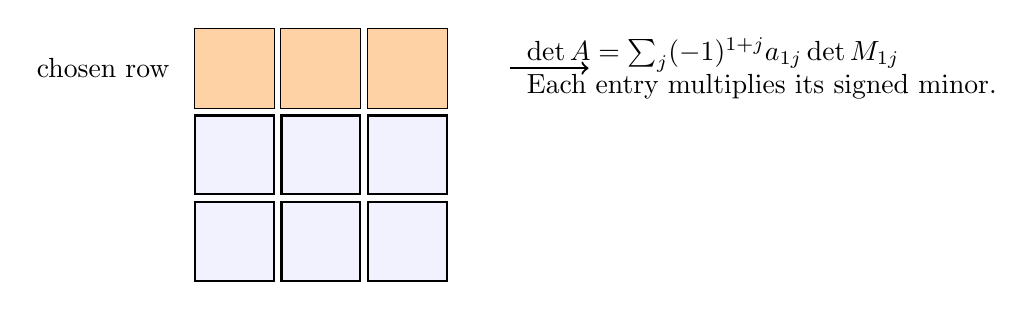
\begin{tikzpicture}
\foreach \i in {0,1,2}{\foreach \j in {0,1,2}{\draw[thick,fill=blue!5] (1.1*\j,-1.1*\i) rectangle +(1,1);}}
\foreach \j in {0,1,2}{\fill[orange!35] (1.1*\j,0) rectangle +(1,1);}
\node[left] at (-.2,.5) {chosen row};
\draw[->,thick] (4,.5)--(5,.5);
\node[align=left] at (7.2,.5) {$\det A=\sum_j(-1)^{1+j}a_{1j}\det M_{1j}$\\Each entry multiplies its signed minor.};
\end{tikzpicture}
